\chapter{Architectural Views for Suggestions to Improve the Existing System}

\section{Context View}

\subsection{Stakeholders' uses of this view}

\subsection{Context Diagram}

\subsection{External Interfaces}

\subsection{Interaction scenarios}

\section{Functional View}

\subsection{Stakeholders' use of this view}

\subsection{Component Diagram}

\subsection{Internal Interfaces}

\subsection{Interaction Patterns}

\section{Information View}
This view focuses on suggestions to make the website better by adding new functionalities to database.

\subsection{Stakeholders' uses of this view}
\begin{itemize}
    \item Volunteers use this view to understand how an outdated, or wrong data is corrected.
    \item Developers use this view to correct wrong and outdated datas.
\end{itemize}

\subsection{Database Class Diagram}
\begin{figure}[H]
    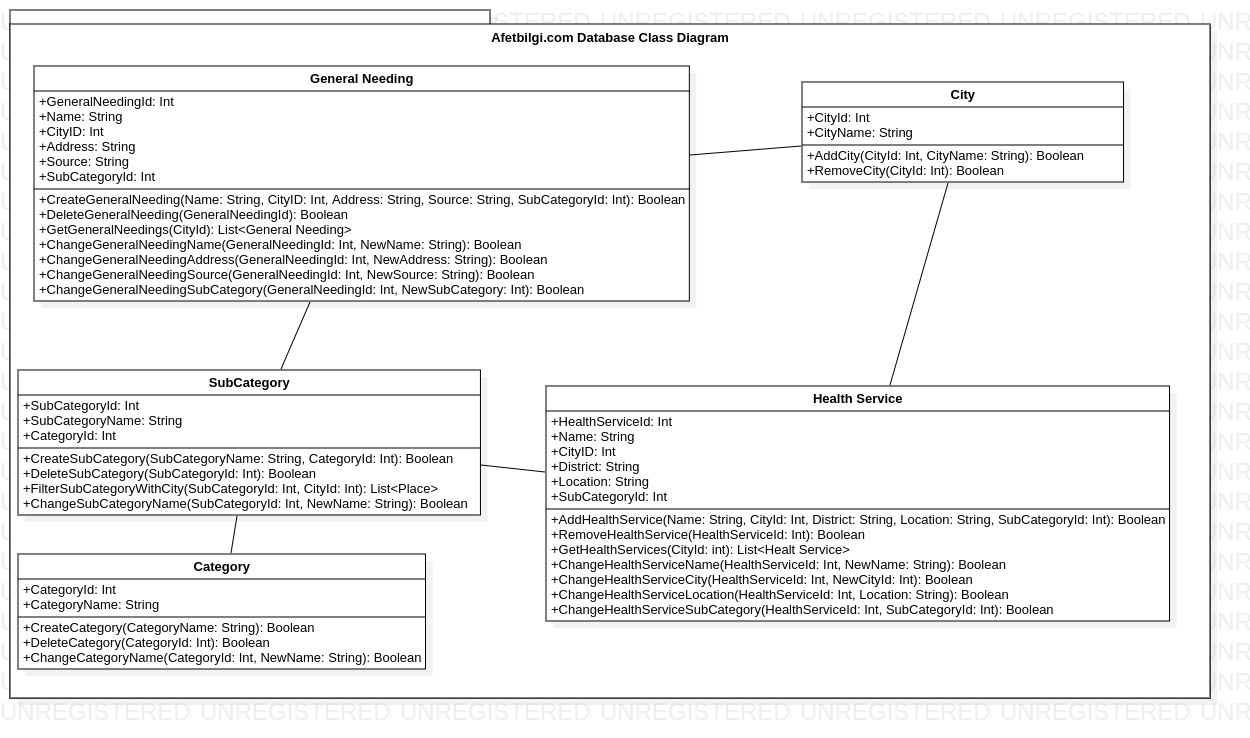
\includegraphics[scale = 0.4]{assets/ClassDiagram2.png}
    \caption[Database Class Diagram With Suggestions]{Database Class Diagram With Suggestions}
\end{figure}

\subsection{Operations on Data}
\begin{table}[H]
    \begin{tabular}{|p{6cm}|p{10cm}|}
        \hline
        \textbf{Operation}   & \textbf{Description}                                                                                                                                    \\
        \hline
        \hline
        ChangeHealthServiceName & Changes name of given healthcare service with given name.\\
        \hline
        ChangeHealthServiceCity & Changes city of given healthcare service.\\
        \hline
        ChangeHealthServiceLocation & Changes location link of given healthcare service. \\
        \hline
        ChangeHealthServiceSubcategory & Changes subcategory of given healthcare service.\\
        \hline
        ChangeSubCategoryname & Change name of subcategory.\\
        \hline
        ChangeGeneralNeedingName & Changes name of general needing.\\
        \hline
        ChangeGeneralNeedingAddress & Changes address link of general needing.\\
        \hline
        ChangeGeneralNeedingSource & Changes source link of general needing.\\
        \hline 
        ChangeGeneralNeedingSubCategory & Changes subcategory of general needing.\\
        \hline
    \end{tabular}
    \caption[Operations on Data with Suggestions]{Operations on Data with Suggestions}
\end{table}


\section{Deployment View}

\subsection{Stakeholders' uses of this view}
\begin{itemize}
    \item Developers can use this view to find out how they can deploy the website when it becomes bigger.
\end{itemize}

\subsection{Deployment Diagram}
\begin{figure}[H]
    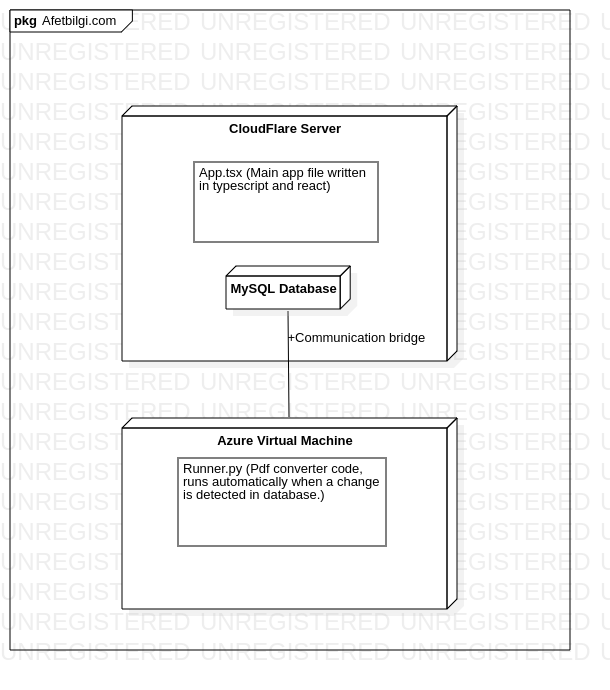
\includegraphics[scale = 0.5]{assets/DeploymentDiagram2.png}
    \caption[Deployment Diagram with Suggestions]{Deployment Diagram with Suggestions}
\end{figure}

\section{Design Rationale}
\begin{itemize}
    \item New data operations should be added to fix and correct datas.
    \item Deployment should be seperated on two services, one for deploying the website and handling SQL database, one for updating pdf constantly. So if one of them crashes users can continue to get information by another.
\end{itemize}